\begin{problem}[Hatcher {\S}2.1, Ex.\@ 20]
Show that $\widetilde H_n(X)\cong\widetilde H_{n+1}(SX)$ for all $n$, where
$SX$ is the suspension of $X$. More generally, thinking of $SX$ as the
union of two cones $CX$ with their bases identified, compute the reduced
homology groups of the union of any finite number of cones $CX$ with their
bases identified.
\end{problem}
\begin{proof}
First note that the reduced suspension of $X$, $\Sigma X$, which is
homotopy equivalent to $SX$, can be realized as the quotient space
$CX/X$. Given the imbedding $X\hookrightarrow CX$, by 2.16 and excision (or
2.22) we have the long exact sequence in
\begin{equation}
\label{eq:suspension-long-exact-sequence}
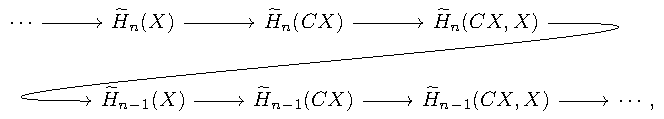
\includegraphics{hw-4-long-exact-sequence-suspension}
\end{equation}
where $\widetilde H_n(CX,X)\cong\widetilde H_n(CX/X)\cong\widetilde
H_n(SX)$. Since $CX$ is contractible, we have $H_n(CX)=0$ for all
$n$ and the long exact sequence \eqref{eq:suspension-long-exact-sequence}
yields an isomorphism
\[
\widetilde H_n(SX)\cong\widetilde H_{n-1}(X).\qedhere
\]
\end{proof}
\newpage

\begin{problem}[Hatcher {\S}2.1, Ex.\@ 22]
Prove by induction on the dimension the following facts about the homology
of a finite dimensional CW complex $X$, using the observation that
$X^n/X^{n-1}$ is a wedge sum of $n$-spheres:
\begin{enumerate}[label=(\alph*)]
\item If $X$ has dimension $n$ then $H_i(X)=0$ for $i>n$ and $H_n(X)$ is
  free.
\item $H_n(X)$ is free with basis in bijective correspondence with the
  $n$-cells if there are no cells of dimension $n-1$ or $n+1$.
\item If $X$ is has $k$ $n$-cells, then $H_n(X)$ is generated by at most
  $k$ elements.
\end{enumerate}
\end{problem}
\begin{proof}
\end{proof}
\newpage

\begin{problem}[Hatcher {\S}2.2, Ex.\@ 2]
Given a map $f\colon S^{2n}\to S^{2n}$, show that there is some point $x\in
S^{2n}$ with either $f(x)=x$ or $f(x)=-x$. Deduce that every map
$\bbRP^{2n}\to\bbRP^{2n}$ has a fixed point. Construct maps
$\bbRP^{2n-1}\to\bbRP^{2n-1}$ without fixed points from linear
transformations $\bbR^{2n}\to\bbR^{2n}$ without eigenvectors.
\end{problem}
\begin{proof}
\end{proof}

%%% Local Variables:
%%% mode: latex
%%% TeX-master: "../MA572-HW-Current"
%%% End:
